\documentclass{article}
\usepackage[utf8]{inputenc}
\usepackage[left=0.7in,top=0.8in,right=0.7in,bottom=1in]{geometry}
\usepackage{amsmath}
\usepackage{hyperref}
\usepackage{graphicx}
\usepackage{longtable}
\usepackage{booktabs}


\title{CS6700 Reinforcement learning\\ Assignment-2}
\author{Arulkumar S (CS15D202)}
\date{\today}

\begin{document}
\maketitle

\section*{Question 1 solutions}

Q 1.1) The implementation of the DP algorithm is submitted in Moodle
\\\\
Q 1.2) 
\subsubsection*{optimal policy for N=10}

\begin{longtable}{|c|c|c|c|}
\toprule
{} &         A &         B &         C \\
\midrule
\endhead
\midrule
\multicolumn{4}{r}{{Continued on next page}} \\
\midrule
\endfoot

\bottomrule
\endlastfoot
\textbf{0 } &  123.0173 &  136.8492 &  124.1938 \\\hline
\textbf{1 } &  109.6728 &  123.5047 &  110.8493 \\\hline
\textbf{2 } &   96.3283 &  110.1602 &   97.5048 \\\hline
\textbf{3 } &   82.9838 &   96.8157 &   84.1602 \\\hline
\textbf{4 } &   69.6394 &   83.4711 &   70.8158 \\\hline
\textbf{5 } &   56.2960 &   70.1263 &   57.4727 \\\hline
\textbf{6 } &   42.9653 &   56.7798 &   44.1377 \\\hline
\textbf{7 } &   29.6641 &   43.4219 &   30.9062 \\\hline
\textbf{8 } &   17.7500 &   29.9375 &   17.8750 \\\hline
\textbf{9 } &    8.0000 &   16.0000 &    7.0000 \\\hline
\textbf{10} &    0.0000 &    0.0000 &    0.0000 \\\hline
\caption{$J_t(s)$ for $t=0 \dots 9 \& s \in [A, B, C]$. Rows correspond to timesteps and Columns correspond to states).}
\end{longtable}


\begin{longtable}{|c|c|c|c|c|c|c|c|c|c|c|c|}
\toprule
{} &  0  &  1  &  2  &  3  &  4  &  5  &  6  &  7  &  8  &  9  & 10 \\
\midrule
\endhead
\midrule
\multicolumn{12}{r}{{Continued on next page}} \\
\midrule
\endfoot

\bottomrule
\endlastfoot
\textbf{A} &   2 &   2 &   2 &   2 &   2 &   2 &   2 &   2 &   1 &   1 &  - \\\hline
\textbf{B} &   2 &   2 &   2 &   2 &   2 &   2 &   2 &   2 &   2 &   1 &  - \\\hline
\textbf{C} &   2 &   2 &   2 &   2 &   2 &   2 &   2 &   2 &   2 &   1 &  - \\\hline
\caption{optimal policy for N=10. Rows correspond to states and Columns correspond to timesteps (N).}
\end{longtable}

\clearpage
\subsubsection*{optimal policy for N=20}

$J_0^*(A) = 256.44, J_0^*(B) = 270.27, J_0^*(C) = 257.62$

\begin{longtable}{|c|c|c|c|}
\toprule
{} &         A &         B &         C \\
\midrule
\endhead
\midrule
\multicolumn{4}{r}{{Continued on next page}} \\
\midrule
\endfoot

\bottomrule
\endlastfoot
\textbf{0 } &  256.4623 &  270.2942 &  257.6388 \\\hline
\textbf{1 } &  243.1178 &  256.9497 &  244.2943 \\\hline
\textbf{2 } &  229.7733 &  243.6052 &  230.9498 \\\hline
\textbf{3 } &  216.4288 &  230.2607 &  217.6053 \\\hline
\textbf{4 } &  203.0843 &  216.9162 &  204.2608 \\\hline
\textbf{5 } &  189.7398 &  203.5717 &  190.9163 \\\hline
\textbf{6 } &  176.3953 &  190.2272 &  177.5718 \\\hline
\textbf{7 } &  163.0508 &  176.8827 &  164.2273 \\\hline
\textbf{8 } &  149.7063 &  163.5382 &  150.8828 \\\hline
\textbf{9 } &  136.3618 &  150.1937 &  137.5383 \\\hline
\textbf{10} &  123.0173 &  136.8492 &  124.1938 \\\hline
\textbf{11} &  109.6728 &  123.5047 &  110.8493 \\\hline
\textbf{12} &   96.3283 &  110.1602 &   97.5048 \\\hline
\textbf{13} &   82.9838 &   96.8157 &   84.1602 \\\hline
\textbf{14} &   69.6394 &   83.4711 &   70.8158 \\\hline
\textbf{15} &   56.2960 &   70.1263 &   57.4727 \\\hline
\textbf{16} &   42.9653 &   56.7798 &   44.1377 \\\hline
\textbf{17} &   29.6641 &   43.4219 &   30.9062 \\\hline
\textbf{18} &   17.7500 &   29.9375 &   17.8750 \\\hline
\textbf{19} &    8.0000 &   16.0000 &    7.0000 \\\hline
\textbf{20} &    0.0000 &    0.0000 &    0.0000 \\\hline
\caption{$J_t(s)$ for $t=0 \dots 19 \& s \in [A, B, C]$. Rows correspond to timesteps and Columns correspond to states).}
\end{longtable}

\begin{longtable}{|c|c|c|c|c|c|c|c|c|c|c|c|c|c|c|c|c|c|c|c|c|c|}
\toprule
{} &  0  &  1  &  2  &  3  &  4  &  5  &  6  &  7  &  8  &  9  &  10 &  11 &  12 &  13 &  14 &  15 &  16 &  17 &  18 &  19 & 20 \\
\midrule
\endhead
\midrule
\multicolumn{22}{r}{{Continued on next page}} \\
\midrule
\endfoot

\bottomrule
\endlastfoot
\textbf{A} &   2 &   2 &   2 &   2 &   2 &   2 &   2 &   2 &   2 &   2 &   2 &   2 &   2 &   2 &   2 &   2 &   2 &   2 &   1 &   1 &  - \\
\textbf{B} &   2 &   2 &   2 &   2 &   2 &   2 &   2 &   2 &   2 &   2 &   2 &   2 &   2 &   2 &   2 &   2 &   2 &   2 &   2 &   1 &  - \\
\textbf{C} &   2 &   2 &   2 &   2 &   2 &   2 &   2 &   2 &   2 &   2 &   2 &   2 &   2 &   2 &   2 &   2 &   2 &   2 &   2 &   1 &  - \\\hline
\caption{optimal policy for N=20. Rows correspond to states and Columns correspond to timesteps (N).}
\end{longtable}
~\\\\

Q 1.3) \textbf{When the policy is to force the driver to go to nearest taxi stand always (i.e., choose action 2 always):}\\

When N = 10, the maximum rewards w.r.t., starting states A, B, C are $J_0^*(A) = 121.5, J_0^*(B) = 135.34, J_0^*(C) = 122.68$ respectively.\\


\begin{longtable}{|c|c|c|c|}
\toprule
{} &         A &         B &         C \\
\midrule
\endhead
\midrule
\multicolumn{4}{r}{{Continued on next page}} \\
\midrule
\endfoot

\bottomrule
\endlastfoot
\textbf{0 } &  121.5003 &  135.3322 &  122.6768 \\\hline
\textbf{1 } &  108.1558 &  121.9877 &  109.3323 \\\hline
\textbf{2 } &   94.8113 &  108.6432 &   95.9878 \\\hline
\textbf{3 } &   81.4668 &   95.2987 &   82.6433 \\\hline
\textbf{4 } &   68.1223 &   81.9542 &   69.2988 \\\hline
\textbf{5 } &   54.7781 &   68.6096 &   55.9546 \\\hline
\textbf{6 } &   41.4360 &   55.2647 &   42.6124 \\\hline
\textbf{7 } &   28.1104 &   41.9170 &   29.2871 \\\hline
\textbf{8 } &   14.9219 &   28.5469 &   16.0938 \\\hline
\textbf{9 } &    2.7500 &   15.0000 &    4.0000 \\\hline
\textbf{10} &    0.0000 &    0.0000 &    0.0000 \\\hline
\caption{$J_t(s)$ for $t=0 \dots 9 \& s \in [A, B, C]$. Rows correspond to timesteps and Columns correspond to states).}
\end{longtable}

When N = 20, the maximum rewards w.r.t., starting states A, B, C are $J_0^*(A) = 254.91, J_0^*(B) = 268.74, J_0^*(C) = 256.09$ respectively.\\

\begin{longtable}{|c|c|c|c|}
\toprule
{} &         A &         B &         C \\
\midrule
\endhead
\midrule
\multicolumn{4}{r}{{Continued on next page}} \\
\midrule
\endfoot

\bottomrule
\endlastfoot
\textbf{0 } &  254.9453 &  268.7772 &  256.1218 \\\hline
\textbf{1 } &  241.6008 &  255.4327 &  242.7773 \\\hline
\textbf{2 } &  228.2563 &  242.0882 &  229.4328 \\\hline
\textbf{3 } &  214.9118 &  228.7437 &  216.0883 \\\hline
\textbf{4 } &  201.5673 &  215.3992 &  202.7438 \\\hline
\textbf{5 } &  188.2228 &  202.0547 &  189.3993 \\\hline
\textbf{6 } &  174.8783 &  188.7102 &  176.0548 \\\hline
\textbf{7 } &  161.5338 &  175.3657 &  162.7103 \\\hline
\textbf{8 } &  148.1893 &  162.0212 &  149.3658 \\\hline
\textbf{9 } &  134.8448 &  148.6767 &  136.0213 \\\hline
\textbf{10} &  121.5003 &  135.3322 &  122.6768 \\\hline
\textbf{11} &  108.1558 &  121.9877 &  109.3323 \\\hline
\textbf{12} &   94.8113 &  108.6432 &   95.9878 \\\hline
\textbf{13} &   81.4668 &   95.2987 &   82.6433 \\\hline
\textbf{14} &   68.1223 &   81.9542 &   69.2988 \\\hline
\textbf{15} &   54.7781 &   68.6096 &   55.9546 \\\hline
\textbf{16} &   41.4360 &   55.2647 &   42.6124 \\\hline
\textbf{17} &   28.1104 &   41.9170 &   29.2871 \\\hline
\textbf{18} &   14.9219 &   28.5469 &   16.0938 \\\hline
\textbf{19} &    2.7500 &   15.0000 &    4.0000 \\\hline
\textbf{20} &    0.0000 &    0.0000 &    0.0000 \\\hline
\caption{$J_t(s)$ for $t=0 \dots 19 \& s \in [A, B, C]$. Rows correspond to timesteps and Columns correspond to states).}
\end{longtable}

Comparing the maximum rewards calculated from Q 1.2, we can observe that always choosing action 2 is not optimal compared to allowing all the actions.

% \begin{longtable}{|c|c|c|c|c|c|c|c|c|c|c|c|}
% \toprule
% {} &        0  &        1  &        2  &       3  &       4  &       5  &       6  &       7  &       8  &     9  &  10 \\
% \midrule
% \endhead
% \midrule
% \multicolumn{12}{r}{{Continued on next page}} \\
% \midrule
% \endfoot

% \bottomrule
% \endlastfoot
% \textbf{A} &  121.5003 &  108.1558 &   94.8113 &  81.4668 &  68.1223 &  54.7781 &  41.4360 &  28.1104 &  14.9219 &   2.75 &   0 \\
% \textbf{B} &  135.3322 &  121.9877 &  108.6432 &  95.2987 &  81.9542 &  68.6096 &  55.2647 &  41.9170 &  28.5469 &  15.00 &   0 \\
% \textbf{C} &  122.6768 &  109.3323 &   95.9878 &  82.6433 &  69.2988 &  55.9546 &  42.6124 &  29.2871 &  16.0938 &   4.00 &   0 \\
% \end{longtable}

\clearpage
\section*{Question 2 solutions}

Q 2.1) From the pseudocode give above, observe that for loop goes on till infinity, so when would you decide to stop value iteration?

\paragraph{Solution: } We can track the maximum change between the value function of any state between each consecutive iterations ($max_s |J_{i+1}(s) - J_i(s)|$). When the change is less than a certain threshold $\epsilon$ (for example, $\epsilon = 1e^{-6}$, we can decide to stop the loop.

\begin{figure}[!htb]
    \centering
    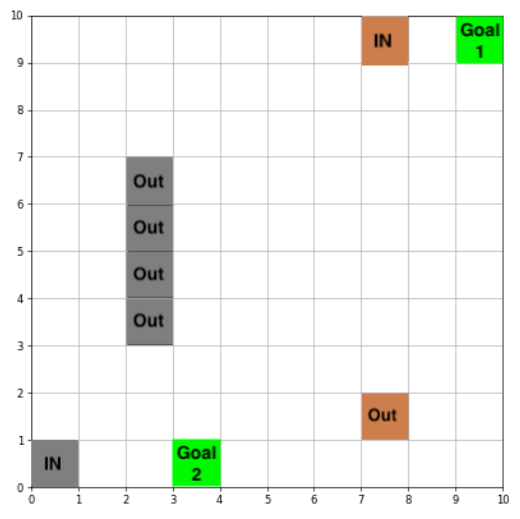
\includegraphics[scale=0.6]{./pics/maze}
    \caption{Maze diagram}
    \label{fig:maze}
\end{figure}

\clearpage
Q 2.2) \textbf{$max_s |J_{i+1}(s) - J_i(s)|$ vs iterations graph}

\begin{figure}[!htb]
    \centering
    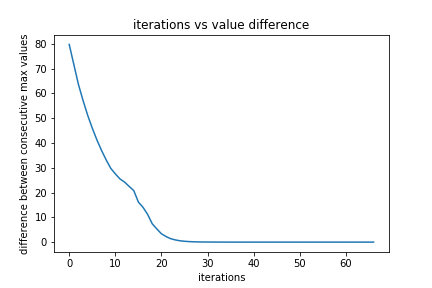
\includegraphics[scale=0.95]{./pics/goal1}
    \label{fig:maze}
    \caption{$max_s |J_{i+1}(s) - J_i(s)|$ vs iterations graph for Goal-1}
\end{figure}

\begin{figure}[!htb]
    \centering
    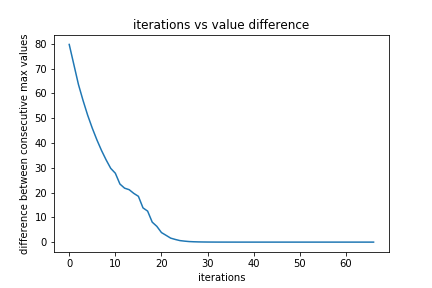
\includegraphics[scale=0.95]{./pics/goal2}
    \caption{$max_s |J_{i+1}(s) - J_i(s)|$ vs iterations graph for Goal-2}
    \label{fig:maze}
\end{figure}

~\\\\
Q 2.3) \textbf{$J(s)$ and Greedy policy 
$\pi(s)$ after iterations 10, 25 and at the end of Value iteration (VI) algorithm }

\subsubsection*{GOAL-1 : After 10th iteration}

\begin{longtable}{|c|c|c|c|c|c|c|c|c|c|c|}
\toprule
{} &       0 &       1 &       2 &       3 &       4 &       5 &       6 &       7 &       8 &       9 \\
\midrule
\endhead
\midrule
\multicolumn{11}{r}{{Continued on next page}} \\
\midrule
\endfoot

\bottomrule
\endlastfoot
\textbf{0} &  15.891 &  44.016 &  62.157 &  79.675 &  87.545 &  93.277 &  95.970 &  98.004 &  99.548 &  \textbf{GOAL} \\\hline
\textbf{1} &  13.045 &  24.836 &  57.150 &  68.072 &  84.209 &  89.186 &  94.236 &  96.357 &  98.179 &  99.548 \\\hline
\textbf{2} & -10.000 &  18.976 &  27.795 &  60.511 &  69.198 &  84.860 &  89.437 &  94.294 &  96.357 &  98.004 \\\hline
\textbf{3} & -10.000 & -10.000 & -10.000 &  28.371 &  60.989 &  70.631 &  84.955 &  89.530 &  94.236 &  95.972 \\\hline
\textbf{4} & -10.000 & -10.000 & -10.000 &  20.803 &  37.731 &  62.474 &  73.794 &  84.920 &  89.411 &  93.279 \\\hline
\textbf{5} & -10.000 & -10.000 & -10.000 &  17.059 &  32.730 &  58.330 &  68.246 &  79.905 &  84.550 &  87.818 \\\hline
\textbf{6} & -10.000 & -10.000 & -10.000 &  26.198 &  56.655 &  67.517 &  82.594 &  86.576 &  83.714 &  81.228 \\\hline
\textbf{7} & -10.000 &  13.723 &  23.315 &  55.083 &  66.679 &  82.637 &  88.477 &  93.482 &  88.760 &  83.766 \\\hline
\textbf{8} &   3.556 &  10.502 &  43.838 &  59.479 &  79.225 &  87.221 &  93.633 &  96.765 &  93.642 &  87.506 \\\hline
\textbf{9} & -10.000 &  13.723 &  34.965 &  61.018 &  75.106 &  85.595 &  90.353 &  93.793 &  90.355 &  85.607 \\\hline
\caption{$J(s)$ 10th iteration}
\end{longtable}

\begin{longtable}{|c|c|c|c|c|c|c|c|c|c|c|}
\toprule
{} &  0 &  1 &  2 &  3 &  4 &  5 &  6 &  7 &  8 &  9 \\
\midrule
\endhead
\midrule
\multicolumn{11}{r}{{Continued on next page}} \\
\midrule
\endfoot

\bottomrule
\endlastfoot
\textbf{0} &  R &  R &  R &  R &  R &  R &  R &  R &  R &  \textbf{GOAL}\\\hline
\textbf{1} &  R &  R &  R &  R &  R &  R &  R &  R &  U &  U \\\hline
\textbf{2} &  U &  R &  U &  R &  R &  R &  R &  U &  U &  U \\\hline
\textbf{3} &  U &  U &  U &  R &  R &  R &  R &  U &  U &  U \\\hline
\textbf{4} &  U &  U &  U &  R &  R &  R &  R &  R &  U &  U \\\hline
\textbf{5} &  D &  R &  U &  R &  R &  R &  D &  D &  U &  U \\\hline
\textbf{6} &  D &  D &  U &  R &  R &  R &  D &  D &  D &  U \\\hline
\textbf{7} &  R &  R &  R &  R &  R &  R &  D &  D &  D &  L \\\hline
\textbf{8} &  R &  R &  R &  R &  R &  R &  R &  U &  L &  L \\\hline
\textbf{9} &  R &  R &  R &  R &  R &  R &  R &  U &  L &  L \\\hline
\caption{Greedy policy $\pi(s)$ after 10th iteration. \textit{U = Up, D = Down, R = Right, L = Left}}
\end{longtable}

\clearpage

\subsubsection*{GOAL-1 : After 25th iteration}

\begin{longtable}{|c|c|c|c|c|c|c|c|c|c|c|}
\toprule
{} &       0 &       1 &       2 &       3 &       4 &       5 &       6 &       7 &       8 &       9 \\
\midrule
\endhead
\midrule
\multicolumn{11}{r}{{Continued on next page}} \\
\midrule
\endfoot

\bottomrule
\endlastfoot
\textbf{0} &  88.650 &  90.029 &  91.392 &  92.744 &  94.098 &  95.457 &  96.825 &  98.203 &  99.594 &   \textbf{GOAL} \\\hline
\textbf{1} &  87.890 &  89.273 &  90.611 &  91.935 &  93.229 &  94.518 &  95.801 &  97.076 &  98.342 &  99.594 \\\hline
\textbf{2} &  86.702 &  87.987 &  89.351 &  90.800 &  92.064 &  93.320 &  94.574 &  95.826 &  97.076 &  98.203 \\\hline
\textbf{3} &  85.347 &  86.441 &  86.074 &  89.634 &  90.870 &  92.103 &  93.336 &  94.574 &  95.801 &  96.825 \\\hline
\textbf{4} &  83.879 &  84.897 &  86.074 &  88.699 &  89.879 &  91.045 &  92.203 &  93.357 &  94.522 &  95.457 \\\hline
\textbf{5} &  83.334 &  84.778 &  86.074 &  88.512 &  89.660 &  90.771 &  91.857 &  92.835 &  93.310 &  94.107 \\\hline
\textbf{6} &  84.643 &  85.995 &  86.074 &  89.411 &  90.650 &  91.887 &  93.125 &  94.151 &  93.236 &  92.898 \\\hline
\textbf{7} &  86.096 &  87.574 &  89.004 &  90.536 &  91.839 &  93.127 &  94.403 &  95.644 &  94.416 &  93.241 \\\hline
\textbf{8} &  87.059 &  88.530 &  89.941 &  91.348 &  92.747 &  94.180 &  95.658 &  97.203 &  95.660 &  94.192 \\\hline
\textbf{9} &  87.169 &  88.495 &  89.770 &  91.009 &  92.221 &  93.407 &  94.561 &  95.674 &  94.561 &  93.408 \\\hline
\caption{$J(s)$ after 25th iteration}
\end{longtable}

\begin{longtable}{|c|c|c|c|c|c|c|c|c|c|c|}
\toprule
{} &  0 &  1 &  2 &  3 &  4 &  5 &  6 &  7 &  8 &  9 \\
\midrule
\endhead
\midrule
\multicolumn{11}{r}{{Continued on next page}} \\
\midrule
\endfoot

\bottomrule
\endlastfoot
\textbf{0} &  R &  R &  R &  R &  R &  R &  R &  R &  R & \textbf{GOAL}  \\\hline
\textbf{1} &  R &  R &  R &  R &  R &  R &  R &  R &  U &  U \\\hline
\textbf{2} &  U &  R &  U &  R &  R &  R &  R &  U &  U &  U \\\hline
\textbf{3} &  U &  U &  U &  R &  R &  R &  R &  U &  U &  U \\\hline
\textbf{4} &  U &  U &  U &  R &  R &  R &  R &  R &  U &  U \\\hline
\textbf{5} &  D &  R &  U &  R &  R &  R &  D &  D &  U &  U \\\hline
\textbf{6} &  D &  D &  U &  R &  R &  R &  D &  D &  D &  U \\\hline
\textbf{7} &  R &  R &  R &  R &  R &  R &  D &  D &  D &  L \\\hline
\textbf{8} &  R &  R &  R &  R &  R &  R &  R &  U &  L &  L \\\hline
\textbf{9} &  R &  R &  R &  R &  R &  R &  R &  U &  L &  L \\\hline
\caption{Greedy policy $\pi(s)$ after 25th iteration. \textit{U = Up, D = Down, R = Right, L = Left}}
\end{longtable}

\subsubsection*{GOAL-1 : After stopping value iteration (after 67th iteration)}

\begin{longtable}{|c|c|c|c|c|c|c|c|c|c|c|}
\toprule
{} &       0 &       1 &       2 &       3 &       4 &       5 &       6 &       7 &       8 &       9 \\
\midrule
\endhead
\midrule
\multicolumn{11}{r}{{Continued on next page}} \\
\midrule
\endfoot

\bottomrule
\endlastfoot
\textbf{0} &  88.723 &  90.060 &  91.402 &  92.748 &  94.099 &  95.457 &  96.825 &  98.203 &  99.594 &  \textbf{GOAL} \\\hline
\textbf{1} &  88.025 &  89.326 &  90.634 &  91.942 &  93.232 &  94.519 &  95.801 &  97.076 &  98.342 &  99.594 \\\hline
\textbf{2} &  86.925 &  88.124 &  89.401 &  90.816 &  92.070 &  93.323 &  94.575 &  95.826 &  97.076 &  98.203 \\\hline
\textbf{3} &  85.790 &  86.708 &  86.294 &  89.663 &  90.884 &  92.108 &  93.338 &  94.575 &  95.801 &  96.825 \\\hline
\textbf{4} &  84.642 &  85.460 &  86.294 &  88.745 &  89.902 &  91.056 &  92.208 &  93.359 &  94.523 &  95.458 \\\hline
\textbf{5} &  84.219 &  85.218 &  86.294 &  88.569 &  89.687 &  90.787 &  91.865 &  92.840 &  93.313 &  94.108 \\\hline
\textbf{6} &  85.344 &  86.369 &  86.294 &  89.448 &  90.669 &  91.895 &  93.128 &  94.152 &  93.239 &  92.901 \\\hline
\textbf{7} &  86.466 &  87.757 &  89.073 &  90.558 &  91.847 &  93.131 &  94.405 &  95.644 &  94.417 &  93.243 \\\hline
\textbf{8} &  87.263 &  88.609 &  89.974 &  91.359 &  92.752 &  94.181 &  95.659 &  97.203 &  95.660 &  94.193 \\\hline
\textbf{9} &  87.294 &  88.548 &  89.790 &  91.017 &  92.224 &  93.408 &  94.562 &  95.675 &  94.562 &  93.410 \\\hline
\caption{$J(s)$ after 67th iteration (after VI stops)}
\end{longtable}

\begin{longtable}{|c|c|c|c|c|c|c|c|c|c|c|}
\toprule
{} &  0 &  1 &  2 &  3 &  4 &  5 &  6 &  7 &  8 &  9 \\
\midrule
\endhead
\midrule
\multicolumn{11}{r}{{Continued on next page}} \\
\midrule
\endfoot

\bottomrule
\endlastfoot
\textbf{0} &  R &  R &  R &  R &  R &  R &  R &  R &  R & \textbf{GOAL}  \\\hline
\textbf{1} &  R &  R &  R &  R &  R &  R &  R &  R &  U &  U \\\hline
\textbf{2} &  U &  R &  U &  R &  R &  R &  R &  U &  U &  U \\\hline
\textbf{3} &  U &  U &  U &  R &  R &  R &  R &  U &  U &  U \\\hline
\textbf{4} &  U &  U &  U &  R &  R &  R &  R &  R &  U &  U \\\hline
\textbf{5} &  D &  R &  U &  R &  R &  R &  D &  D &  U &  U \\\hline
\textbf{6} &  D &  D &  U &  R &  R &  R &  D &  D &  D &  U \\\hline
\textbf{7} &  R &  R &  R &  R &  R &  R &  D &  D &  D &  L \\\hline
\textbf{8} &  R &  R &  R &  R &  R &  R &  R &  U &  L &  L \\\hline
\textbf{9} &  R &  R &  R &  R &  R &  R &  R &  U &  L &  L \\\hline
\caption{Greedy policy $\pi(s)$ after 67th iteration (after VI stops)\label{tab:greedypolicy-goal1}. \textit{U = Up, D = Down, R = Right, L = Left}}
\end{longtable}

\subsubsection*{GOAL-2 : After 10th iteration}


\begin{longtable}{|c|c|c|c|c|c|c|c|c|c|c|}
\toprule
{} &       0 &       1 &       2 &       3 &       4 &       5 &       6 &       7 &       8 &       9 \\
\midrule
\endhead
\midrule
\multicolumn{11}{r}{{Continued on next page}} \\
\midrule
\endfoot

\bottomrule
\endlastfoot
\textbf{0} &  33.800 &  54.360 &  59.901 &  54.389 &  29.286 &  14.067 & -10.000 & -10.000 & -10.000 & -10.000 \\\hline
\textbf{1} &  57.935 &  69.377 &  79.490 &  68.973 &  55.677 &  28.046 &  13.935 & -10.000 & -10.000 & -10.000 \\\hline
\textbf{2} &  71.730 &  83.352 &  88.425 &  83.338 &  69.571 &  55.395 &  27.756 &  12.028 & -10.000 & -10.000 \\\hline
\textbf{3} &  82.675 &  89.794 &  94.507 &  89.841 &  82.759 &  68.464 &  51.047 &  25.464 &   3.556 & -10.000 \\\hline
\textbf{4} &  85.145 &  91.061 &  94.507 &  91.148 &  86.297 &  75.900 &  62.608 &  36.618 &  20.775 & -10.000 \\\hline
\textbf{5} &  86.113 &  91.274 &  94.507 &  92.870 &  88.639 &  84.692 &  69.561 &  60.786 &  27.827 &  20.559 \\\hline
\textbf{6} &  87.600 &  91.604 &  94.507 &  95.251 &  94.066 &  89.116 &  84.755 &  67.940 &  59.309 &  29.089 \\\hline
\textbf{7} &  91.449 &  94.378 &  96.303 &  97.678 &  96.242 &  94.230 &  89.144 &  74.996 &  59.989 &  51.912 \\\hline
\textbf{8} &  94.328 &  96.355 &  98.153 &  99.382 &  98.152 &  96.293 &  94.178 & -10.000 &  62.634 &  59.353 \\\hline
\textbf{9} &  96.029 &  97.993 &  99.543 &   \textbf{GOAL} &  99.542 &  97.991&  95.927 &  82.604 &  77.080 &  69.757 \\\hline
\caption{$J(s)$ after 10th iteration}
\end{longtable}


\begin{longtable}{|c|c|c|c|c|c|c|c|c|c|c|}
\toprule
{} &  0 &  1 &  2 &  3 &  4 &  5 &  6 &  7 &  8 &  9 \\
\midrule
\endhead
\midrule
\multicolumn{11}{r}{{Continued on next page}} \\
\midrule
\endfoot

\bottomrule
\endlastfoot
\textbf{0} &  D &  D &  D &  D &  L &  D &  U &  U &  U &  U \\\hline
\textbf{1} &  D &  D &  D &  D &  D &  L &  L &  U &  U &  U \\\hline
\textbf{2} &  D &  D &  D &  D &  L &  L &  L &  L &  U &  U \\\hline
\textbf{3} &  R &  R &  U &  L &  L &  L &  L &  L &  L &  U \\\hline
\textbf{4} &  R &  R &  U &  L &  L &  L &  L &  L &  L &  U \\\hline
\textbf{5} &  R &  R &  U &  D &  D &  D &  L &  L &  L &  L \\\hline
\textbf{6} &  D &  R &  U &  D &  D &  D &  L &  L &  L &  D \\\hline
\textbf{7} &  D &  D &  D &  D &  D &  D &  L &  L &  L &  L \\\hline
\textbf{8} &  R &  R &  D &  D &  D &  L &  L &  U &  D &  D \\\hline
\textbf{9} &  R &  R &  R &  \textbf{GOAL} &  L &  L &  L &  L &  L &  L \\\hline
\caption{Greedy policy $\pi(s)$ after 10th iteration. \textit{U = Up, D = Down, R = Right, L = Left}}
\end{longtable}

\clearpage
\subsubsection*{GOAN-2 : After 25th iteration}

\begin{longtable}{|c|c|c|c|c|c|c|c|c|c|c|}
\toprule
{} &       0 &       1 &       2 &       3 &       4 &       5 &       6 &       7 &       8 &       9 \\
\midrule
\endhead
\midrule
\multicolumn{11}{r}{{Continued on next page}} \\
\midrule
\endfoot

\bottomrule
\endlastfoot
\textbf{0} &  89.702 &  90.620 &  91.362 &  90.574 &  89.455 &  88.303 &  87.113 &  85.846 &  84.467 &  82.846 \\\hline
\textbf{1} &  90.845 &  91.899 &  92.809 &  91.876 &  90.641 &  89.390 &  88.118 &  86.812 &  85.399 &  83.841 \\\hline
\textbf{2} &  91.967 &  93.169 &  94.291 &  93.168 &  91.904 &  90.629 &  89.341 &  88.019 &  86.649 &  85.132 \\\hline
\textbf{3} &  93.069 &  94.430 &  95.822 &  94.437 &  93.084 &  91.754 &  90.434 &  89.113 &  87.760 &  86.349 \\\hline
\textbf{4} &  93.289 &  94.559 &  95.822 &  94.627 &  93.454 &  92.266 &  91.059 &  89.830 &  88.569 &  87.252 \\\hline
\textbf{5} &  93.353 &  94.583 &  95.822 &  95.259 &  94.447 &  93.290 &  92.066 &  90.822 &  89.555 &  88.235 \\\hline
\textbf{6} &  93.582 &  94.698 &  95.822 &  96.540 &  95.741 &  94.551 &  93.301 &  91.943 &  90.564 &  89.150 \\\hline
\textbf{7} &  94.693 &  95.824 &  97.041 &  97.980 &  97.040 &  95.809 &  94.555 &  92.272 &  90.833 &  89.360 \\\hline
\textbf{8} &  95.802 &  97.063 &  98.326 &  99.465 &  98.326 &  97.062 &  95.787 &  84.674 &  90.338 &  89.439 \\\hline
\textbf{9} &  96.822 &  98.200 &  99.592 &   \textbf{GOAL} &  99.592 &  98.200 &  96.820 &  94.318 &  92.662 &  90.970 \\\hline
\caption{$J(s)$ after 25th iteration}
\end{longtable}

\begin{longtable}{|c|c|c|c|c|c|c|c|c|c|c|}
\toprule
{} &  0 &  1 &  2 &  3 &  4 &  5 &  6 &  7 &  8 &  9 \\
\midrule
\endhead
\midrule
\multicolumn{11}{r}{{Continued on next page}} \\
\midrule
\endfoot

\bottomrule
\endlastfoot
\textbf{0} &  D &  D &  D &  D &  L &  L &  L &  L &  L &  L \\\hline
\textbf{1} &  D &  D &  D &  D &  D &  L &  L &  L &  L &  L \\\hline
\textbf{2} &  D &  D &  D &  D &  L &  L &  L &  L &  L &  L \\\hline
\textbf{3} &  R &  R &  U &  L &  L &  L &  L &  L &  L &  L \\\hline
\textbf{4} &  R &  R &  U &  L &  L &  L &  L &  L &  L &  L \\\hline
\textbf{5} &  R &  R &  U &  D &  D &  D &  L &  L &  L &  L \\\hline
\textbf{6} &  D &  R &  U &  D &  D &  D &  L &  L &  L &  L \\\hline
\textbf{7} &  D &  D &  D &  D &  D &  D &  L &  L &  L &  L \\\hline
\textbf{8} &  R &  R &  D &  D &  D &  L &  L &  U &  D &  D \\\hline
\textbf{9} &  R &  R &  R &  \textbf{GOAL} &  L &  L &  L &  L &  L &  L \\\hline
\caption{Greedy policy $\pi(s)$ after 25th iteration. \textit{U = Up, D = Down, R = Right, L = Left}}
\end{longtable}

\subsubsection*{GOAL-2 : After the execution of full value iteration (after 67th iteration)}

\begin{longtable}{|c|c|c|c|c|c|c|c|c|c|c|}
\toprule
{} &       0 &       1 &       2 &       3 &       4 &       5 &       6 &       7 &       8 &       9 \\
\midrule
\endhead
\midrule
\multicolumn{11}{r}{{Continued on next page}} \\
\midrule
\endfoot

\bottomrule
\endlastfoot
\textbf{0} &  89.717 &  90.631 &  91.372 &  90.593 &  89.489 &  88.372 &  87.242 &  86.103 &  84.955 &  83.800 \\\hline
\textbf{1} &  90.852 &  91.903 &  92.812 &  91.884 &  90.660 &  89.430 &  88.207 &  86.988 &  85.772 &  84.558 \\\hline
\textbf{2} &  91.971 &  93.171 &  94.292 &  93.170 &  91.911 &  90.648 &  89.384 &  88.122 &  86.863 &  85.607 \\\hline
\textbf{3} &  93.071 &  94.431 &  95.822 &  94.438 &  93.087 &  91.761 &  90.454 &  89.161 &  87.878 &  86.603 \\\hline
\textbf{4} &  93.290 &  94.559 &  95.822 &  94.628 &  93.456 &  92.270 &  91.069 &  89.855 &  88.632 &  87.401 \\\hline
\textbf{5} &  93.354 &  94.584 &  95.822 &  95.260 &  94.448 &  93.293 &  92.072 &  90.839 &  89.598 &  88.350 \\\hline
\textbf{6} &  93.583 &  94.699 &  95.822 &  96.541 &  95.741 &  94.552 &  93.304 &  91.962 &  90.633 &  89.320 \\\hline
\textbf{7} &  94.694 &  95.824 &  97.042 &  97.980 &  97.040 &  95.809 &  94.556 &  92.352 &  91.031 &  89.789 \\\hline
\textbf{8} &  95.802 &  97.063 &  98.326 &  99.465 &  98.326 &  97.062 &  95.787 &  85.103 &  90.865 &  90.323 \\\hline
\textbf{9} &  96.822 &  98.200 &  99.592 &   \textbf{GOAL} &  99.592 &  98.200 &  96.820 &  94.407 &  92.903 &  91.505 \\\hline
\caption{$J(s)$ after 67th iteration (after VI stops)}
\end{longtable}


\begin{longtable}{|c|c|c|c|c|c|c|c|c|c|c|}
\toprule
{} &  0 &  1 &  2 &  3 &  4 &  5 &  6 &  7 &  8 &  9 \\
\midrule
\endhead
\midrule
\multicolumn{11}{r}{{Continued on next page}} \\
\midrule
\endfoot

\bottomrule
\endlastfoot
\textbf{0} &  D &  D &  D &  D &  L &  L &  L &  L &  L &  L \\\hline
\textbf{1} &  D &  D &  D &  D &  D &  L &  L &  L &  L &  L \\\hline
\textbf{2} &  D &  D &  D &  D &  L &  L &  L &  L &  L &  L \\\hline
\textbf{3} &  R &  R &  U &  L &  L &  L &  L &  L &  L &  L \\\hline
\textbf{4} &  R &  R &  U &  L &  L &  L &  L &  L &  L &  L \\\hline
\textbf{5} &  R &  R &  U &  D &  D &  D &  L &  L &  L &  L \\\hline
\textbf{6} &  D &  R &  U &  D &  D &  D &  L &  L &  L &  L \\\hline
\textbf{7} &  D &  D &  D &  D &  D &  D &  L &  L &  L &  L \\\hline
\textbf{8} &  R &  R &  D &  D &  D &  L &  L &  U &  D &  D \\\hline
\textbf{9} &  R &  R &  R &  \textbf{GOAL} &  L &  L &  L &  L &  L &  L \\\hline
\caption{Greedy policy $\pi(s)$ after 67th iteration (after VI stops) \label{tab:greedypolicy-goal2}. \textit{U = Up, D = Down, R = Right, L = Left}}
\end{longtable}

Q 2.4) \textbf{The behavior of $J$ and Greedy policy $\pi$}

Observing the tables \ref{tab:greedypolicy-goal2}, \ref{tab:greedypolicy-goal1}, we can observe the following behavior of the greedy policy:

\begin{itemize}
    \item In the states far away from the GOAL, but nearby to IN states, the greedy policy chooses to reach IN states as soon as possible (that have connection to the state nearest to the GOAL), so that the reward is maximized.
    
    \item In the states near the GOAL and far away from IN states, the greedy policy chooses to directly move towards GOAL withput going to IN states (which is intuitive to maximize the return)
    
    \item The states nearby the GOAL state has the highest reward among other states.
\end{itemize}

\end{document}